\documentclass[11pt,a5paper]{article}

\usepackage[T1]{fontenc} % font encoding, lubab õ tähte kasutada
\usepackage[utf8]{inputenc} % oleme siiski 21. sajandis, vajadusel on ka olemas utf8x
\usepackage{lmodern, microtype} % lmodern ja micrtype käivad käsikäes, teeb teksti ilusamaks
\usepackage{enumerate}
\usepackage{caption}
\usepackage[estonian]{babel} % eesti keele poolitamisreeglid jpm
\usepackage[per = fraction, expproduct=cdot, decimalsymbol=comma]{siunitx} % http://www.bakoma-tex.com/doc/latex/siunitx/siunitx.pdf
\usepackage{graphicx} 
\usepackage[european]{circuitikz}
\usepackage{wrapfig}
\usepackage{tikz}
\usetikzlibrary{decorations.pathreplacing, positioning}
\usetikzlibrary{arrows,calc,decorations.markings,math,arrows.meta}
\usepackage{siunitx}
\usepackage{epstopdf} %minul on vaja, et .eps pilte saada
%paneme kõik mõõdud paika
\topmargin=-2.5cm \textheight=18cm \textwidth=12.77cm
\oddsidemargin=-1.5cm  \evensidemargin=-1.5cm
\setlength{\parindent}{0pt} \setlength{\parskip}{6pt} \sloppy
\relpenalty=10000 \binoppenalty=10000 % Tekstisisestes valemites reavahetusi ärgu olgu
\pagestyle{empty} % ilma leheküljenumbrita
\newcommand{\numb}[1]{\vspace{5pt}\textbf{\large #1}}
\newcommand{\nimi}[1]{(\textsl{\small #1})}
\newcommand{\punktid}[1]{(\emph{#1~p.})}
\newcommand{\autor}[1]{\emph{ Autor: #1}}
\newcounter{ylesanne}
\newcommand{\yl}[1]{\addtocounter{ylesanne}{1}\numb{\theylesanne.} \nimi{#1} \newblock{}}

\begin{document}

\begin{center}
\textbf{\Large Eesti koolinoorte 30. füüsika lahtine võistlus} \vspace{3pt}

\emph{23. november 2019. a. \\Vanema rühma ülesanded (11. - 12. klass)}\vspace{2pt}\\
\emph{\textbf{Palun kirjutage iga ülesande lahendus eraldi lehele!}}
\end{center}
\vspace{-5pt}

\yl{RISTMIK}
Juku, sõites autoga ($v = \SI{90}{\kilo\meter\per\hour}$), läheneb Y-kujulisele ristmikule. Kui tal on ristmikuni jäänud veel $l = \SI{150}{\meter}$ märkab Juku, et kõrvalharu pealt sõidab ristmiku poole ka teine auto, mille ristmikuni jäänud vahemaa ja kiiruse projektsioonid Juku sõidusuunale on võrdsed Juku auto omadega. Kokkupõrke vältimiseks kiirendab Juku kiirendusega $a = \SI{0.5}{\meter\per\second\squared}$. Mis on autode vahemaa, kui teine auto jõuab ristmikuni? Teede vaheline nurk on \ang{15}.
\punktid{6} \autor{Markus Rene Pae}

\begin{wrapfigure}[7]{r}{0.45\textwidth}
    \vspace{-23pt}
	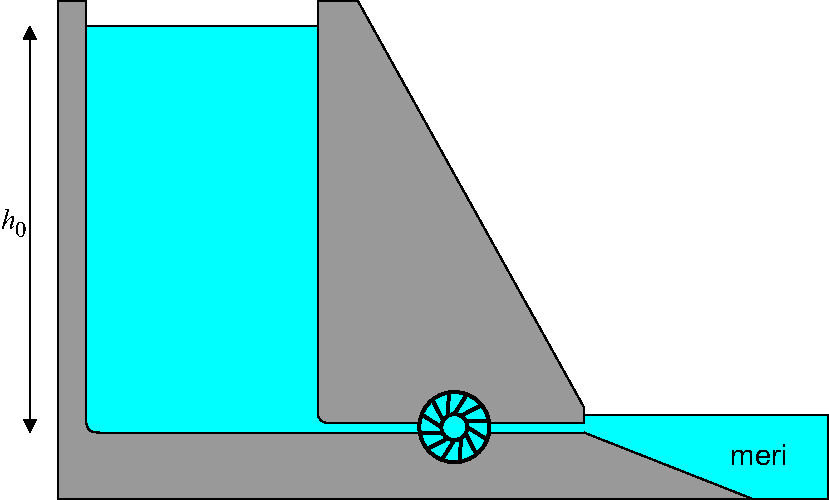
\includegraphics[width=0.45\textwidth]{pumpjaama_joonis.pdf}
\end{wrapfigure}

\yl{PUMPJAAM}
Arenenud riikides on elektrienergia tarbimine, võrrelduna riigi pindalaga, suurusjärgus \SI{100}{\kilo\watt\per\kilo\meter\squared}. Joonisel on kujutatud teatava pump-hüdroakumulatsiooni elektrijaama skeem. Eeldame, et alumiseks reservuaariks on meri (mille tase püsib praktiliselt muutumatu) ja ülemise reservuaari põhi ulatub praktiliselt merepinna tasemeni. Elektrienergia ületootmise ajal pumbatakse merevett ülemisse reservuaari kuni kõrguseni $h_0=\SI{100}{m}$. Energiadefitsiidi ajal toimib sama süsteem hüdroelektrijaamana. Ignoreerides energia konverteerimis- ja ülekandekadusid, kui suure osa riigi pindalast peaks sellised pumpjaamad (st ülemise reservuaari pindala) moodustama, et muude elektritootjate äralangemisel kindlustada elektrienergia varu 24 tunniks?
\punktid{6} \autor{Valter Kiisk}

\yl{LÄÄTS}
Optiline süsteem koosneb punktvalgusallikast ja ekraanist, mille vahele on asetatud õhuke koondav lääts. Ekraani ja valgusallika vaheline kaugus on $L$. Millist tingimust peab rahuldama läätse fookuskaugus, et ekraanile tekiks tõeline kujutis? Kui fookuskaugus on võimalikult suur, siis milline on optilise süsteemi suurendus?
\punktid{8} \autor{Hans Daniel Kaimre}

\yl{LAETUD TASAND}
Ruumis on ühtlaselt laetud tasand ja paaritu arv võrdseid laenguid, mis ei asu tasandil. Tõesta, et tasandile mõjuv resultantjõud ei saa olla 0.
\punktid{8} \autor{Kaarel Hänni}

\yl{KUULID}
Mängupüssist lastakse otse üles kummist kuul algkiirusega $v$. Sel ajal, kui esimene kuul on õhus, lastakse aja $t$ pärast üles teine samasugune kuul samuti algkiirusega $v$. Kui kõrgele $h$ põrkab esimene kuul pärast esimest elastset põrget?
\punktid{10} \autor{Erkki Tempel}

\begin{wrapfigure}[7]{r}{0.5\textwidth}
	\vspace{-24pt}
	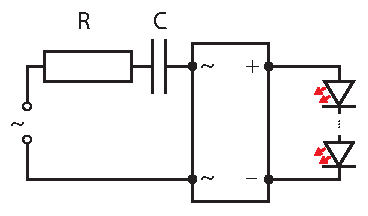
\includegraphics[width=0.5\textwidth]{LED_joonis.pdf}
\end{wrapfigure}

\yl{LED}
LED-lamp koosneb $N=10$-st valgusdioodist (nimipinge $U_{D}=\SI{3.0}{V}$ ja -vool $I_{D}=\SI{100}{mA}$), mida toidetakse vahelduvvooluga (pinge maksimumväärtus $U=\SI{320}{V}$ ja sagedus $f=\SI{50}{Hz}$) läbi takisti ($R=\SI{400}{\ohm}$), kondensaatori ja alaldi (lugeda ideaalseks). Kui suur peab olema kondensaatori mahtuvus $C,$ et valgusdioodid põleksid võimalikult heledalt, kuid ei põleks läbi? Märkus: Takisti ja kondensaatori näivtakistus on $Z=\sqrt{R^{2}+X_{C}^{2}}$, kus $X_{C}=1/\left(2\pi fC\right)$ ning võib eeldada sinusoidaalset voolu ja pinget aladi ees. 
\punktid{10} \autor{Ardi Loot}

\begin{wrapfigure}[7]{r}{0.3\textwidth}
	\vspace{-13pt}
	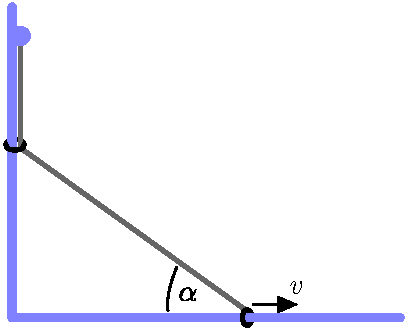
\includegraphics[width=0.3\textwidth]{niit_relsil.pdf}
\end{wrapfigure}

\yl{NIIT RELSSIDEL}
Niit kogupikkusega $L$ on kinnitatud kahest üksteisega ristuvast lõigust koosneva relsi külge nii, nagu näidatud joonisel: üks ots on fikseeritud jäigalt vertikaalse relsiosa külge kaugusele $h$ relsi nurgast, alumine ots tillukese rõnga abil horisontaalse relsi külge. Niit on tõmmatud läbi teise tillukese rõnga, mis saab libiseda mööda vertikaalset relssi. Alumist rõngast liigutatakse konstantse kiirusega $v$. Leida teise rõnga kiirus ja kiirendus hetkel, mil nöör moodustab nurga $\alpha$ horisontaalsihiga.
\punktid{12} \autor{Jaan Kalda}

\yl{KÜLM GAAS}
Tihedalt suletud anumas on monomolekulaarne gaas molaarmassiga $\mu$ ja tihedusega $\rho$ temperatuuril $T_0$. Anum on silindriline ja tema telg vertikaalne. Anum liigub ülevalt alla algkiirusega $v$ ja peatub hetkeliselt; eeldada, et $v\gg \sqrt{RT_0/\mu}$, $R$ tähistab universaalset gaasikonstanti. Millist rõhku avaldab gaas anuma põhjale (a) vahetult peale anuma seinte peatumist; (b) peale seda, kui gaas jõuab termodünaamilisse tasakaalu. Gaasi soojusvahetust anuma seintega ignoreerida, eeldada, et põrkumisel seintega on molekulide eemaldumisnurk pinnanormaali suhtes võrdne langemisnurgaga.
\punktid{12} \autor{Jaan Kalda}

\yl{HANTEL}
Kaks metallkera raadiusega $R$ ja massiga $m$ on ühendatud koaksiaalselt metallvardaga, mille pikkus $L$ on hulga suurem $R$-st ja mille mass ning diameeter on tühiselt väiksed. Kogu süsteem asub kaalutuse tingimustes teljega ristsihilises homogeenses magnetväljas induktsiooniga $B$. Ühele kuulikestest kantakse hetkeliselt elektrilaeng $Q$; visandage ühel ja samal joonisel mõlema kuulikese trajektoorid edasise liikumise käigus. Eeldada, et varda elektriline takistus on tühiselt väike ja et $\varepsilon_0B^2L^2R\ll m$, kus $\varepsilon_0$ tähistab vaakumi dielektrilist läbitavust.
\punktid{14} \autor{Jaan Kalda}


\yl{LAME MAA}
Juku lendab lennukiga $h=\SI{10}{km}$ kõrgusel, suunab kaamera optilise peatelje horisondile ja teeb pildi. Seejärel trükib ta pildi 10x10 cm paberile ($L=\SI{10}{cm}$). Kui palju on pildi servas horisont maakera kumeruse tõttu madalamal kui pildi keskel? Võib eeldada, et see suurus on väga väike. Kaamera vaatenurk $2\beta=\SI{50}{\degree}$, Maa raadius $R=\SI{6000}{km}$. \punktid{14} \autor{Andres Põldaru}



\end{document}